\begin{frame}[fragile]

  \frametitle{Fault Tolerance in Charm++/AMPI}

  \begin{itemize}
    \item Four Approaches:

      \begin{itemize}
\item Disk-based checkpoint/restart
\item In-memory double checkpoint/restart
\item Experimental: Proactive object migration 
\item Experimental: Message-logging for scalable fault tolerance
      \end{itemize}
    \item Common Features:
\begin{itemize}
\item Easy checkpoint 
\item Migrate-to-disk leverages object-migration capabilities
\item Based on dynamic runtime capabilities
\item Can be used in concert with load-balancing schemes
     \end{itemize}
  \end{itemize}
\end{frame}

\begin{frame}[fragile]
  \frametitle{Checkpointing to the file system : Split Execution}
\begin{itemize}
\item The common form of checkpointing
\begin{itemize}
\item The job runs for 5 hours, then will continue at the next
  allocation another day! 
\end{itemize}

\item The existing Charm++ infrastructure for chare migration helps
\item Just ``migrate'' chares to disk
\item The call to checkpoint the application is made in the main chare at a synchronization point
\end{itemize}

 \begin{lstlisting}[basicstyle=\footnotesize]

      CkCallback cb(CkIndex_Hello::SayHi(),helloProxy);
      CkStartCheckpoint(``log'',cb);

> ./charmrun hello +p4 +restart log

\end{lstlisting}

\end{frame}

\begin{frame}[fragile]
  \frametitle{In-memory checkpointing with auto restart}
\begin{itemize}

\item Idea: checkpoint data in a buddy processor's memory, in addition
  to a local checkpoint
\item System auto detects when a node crashes
\item  Failed process is restarted on a spare, and retrieves it
  checkpoint form the buddy
\item (you can also do without the spare)
\item Every other processor retrieves its local checkpoint 
\end{itemize}

 \begin{lstlisting}[basicstyle=\footnotesize]

void CkStartMemCheckpoint(CkCallback &cb)
\end{lstlisting}

\end{frame}

\begin{frame}[fragile]
  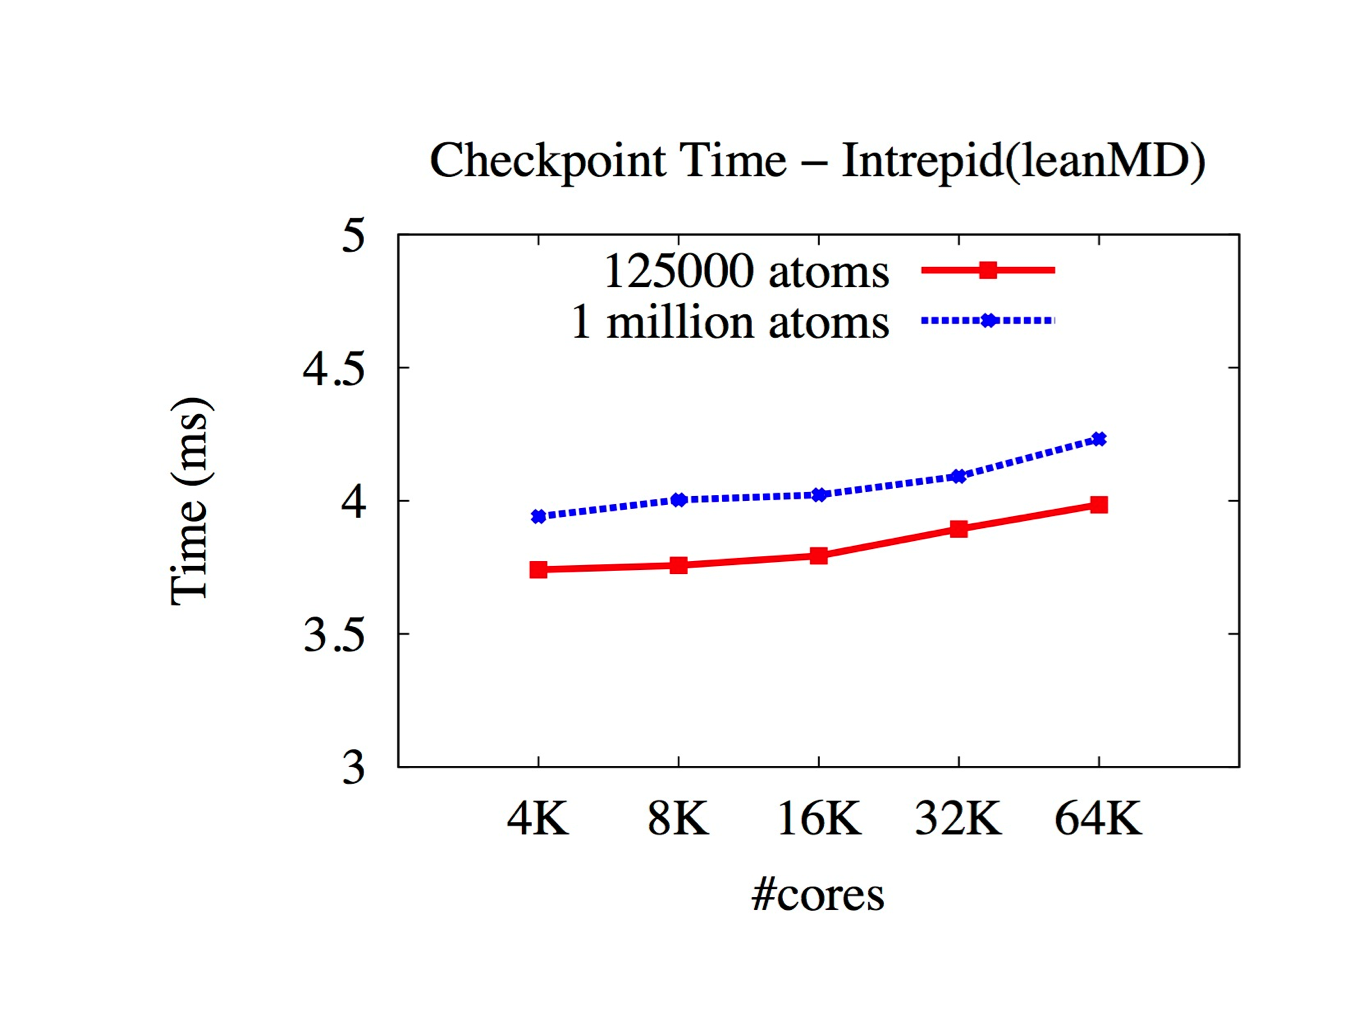
\includegraphics[width=\textwidth]{figures/checkpointTimeIntrepid.png}
\end{frame}

\begin{frame}[fragile]
  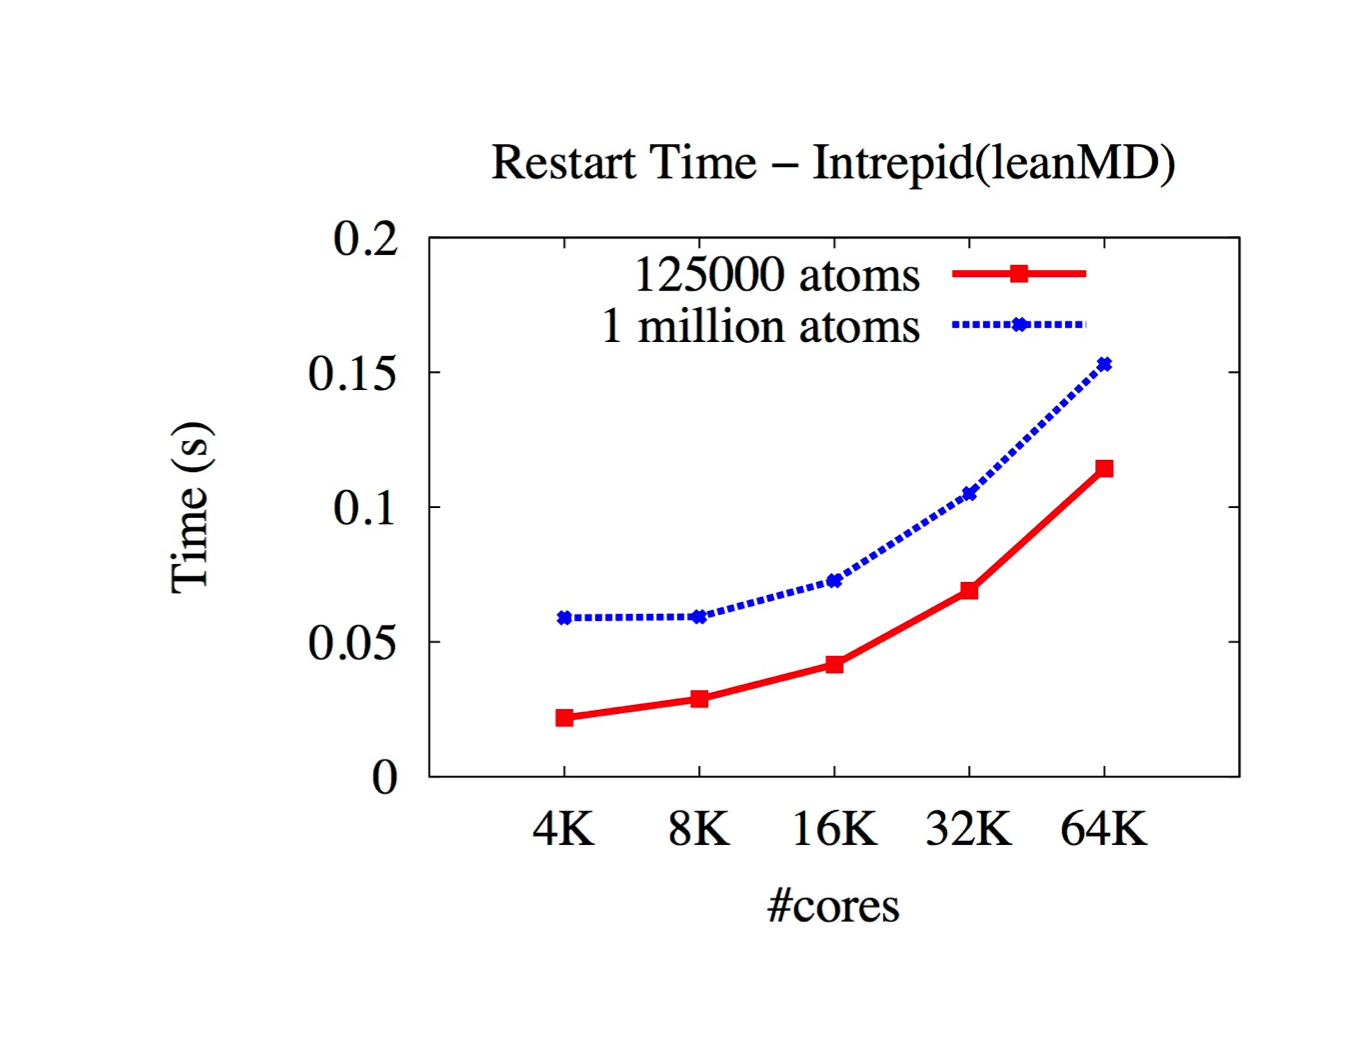
\includegraphics[width=\textwidth]{figures/restartTimeIntrepid.png}
\end{frame}

